%% beamerexample.tex
  %% Copyright 2012 Kartik Prabhu <kartikprabhu00@gmail.com>
  %
  % This work may be distributed and/or modified under the
  % conditions of the LaTeX Project Public License, either version 1.3
  % of this license or (at your option) any later version.
  % The latest version of this license is in
  %   http://www.latex-project.org/lppl.txt
  % and version 1.3 or later is part of all distributions of LaTeX
  % version 2005/12/01 or later.
  %
  % Or see the file LPPL-license for more details.
  % 
  


\documentclass{beamer} 

\usepackage{amsmath,amssymb,amsfonts,dcolumn,color,graphicx,graphics,setspace,latexsym,setspace,lscape,subfigure,placeins,epsfig,hyperref}
\usepackage{eulervm}
 

\usetheme{Kalgan}


\setbeamercovered{highly dynamic}
\setbeamersize{text margin left=10pt}

\newcommand{\be}{\begin{equation}}
\newcommand{\ee}{\end{equation}}
\newcommand{\lb}{\left}
\newcommand{\rb}{\right}





\title{Beamer Example}
\author{Li Europan}
\institute[LI]{LoremIpsum}
\date{}

\begin{document}

	\begin{frame}[plain]
	  \titlepage
	\end{frame}
	\begin{frame}
  		\frametitle{Outline}
		\tableofcontents
	\end{frame}
	
	\section{Just some Text}
		\begin{frame}
			\frametitle{Here is some text}
				\begin{itemize}[<+->]
				\item This is some normal text.\\
				\item This is some \alert{alerted text.}\\
				\item This is some inline math $e^{i\pi} + 1 =0$
				\item This is some displayed math
						\be
							f^{(n)}(z_0) = \frac{n!}{2\pi i}\oint_C \frac{f(z)}{(z-z_0)^{n+1}} dz
						\ee
				 \begin{quotation}
				  This is a quotation.
				 \end{quotation}
			\end{itemize}
		\end{frame}

	\section{Blocks and Columns}
		\subsection{Blocks}
			\begin{frame}
	 		\frametitle{Blocks}
			   \begin{block}{This is a Block}
			      This is important information
			   \end{block}
			 
			   \begin{alertblock}{This is an Alert block}
			   This is an important alert
			   \end{alertblock}

			   \begin{exampleblock}{This is an Example block}
			   This is an example 
			   \end{exampleblock}
			\end{frame}
		
		\subsection{Columns}
			\begin{frame}
		    \begin{columns}[c] % the "c" option specifies center vertical alignment
		    \column{.5\textwidth} % column designated by a command
		     Contents of the first column
		    \column{.5\textwidth}
		     Contents split \\ into two lines
		    \end{columns}
		\end{frame}
		 
		\begin{frame}
		     \begin{columns}[t] % contents are top vertically aligned
		     \begin{column}[T]{5cm} % each column can also be its own environment
		     Contents of first column \\ split into two lines or more. \\ The chick graphic is from \cite{Chick}. 
		     \end{column}
		     \begin{column}[T]{5cm} % alternative top-align that's better for graphics
		          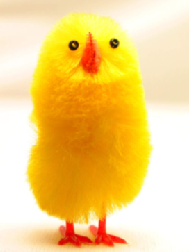
\includegraphics[height=3cm]{Chick1.png}
		     \end{column}
		     \end{columns}
		\end{frame}
		
	\section{Tables \& Figures}
		\subsection{Tables}
		\begin{frame}
			\frametitle{Tables}
				 \begin{table}
				 	\begin{tabular}{ l | c || r | }
					    \hline
					    1 & 2 & 3 \\ \hline
					    4 & 5 & 6 \\ \hline
					    7 & 8 & 9 \\
					    \hline
					  \end{tabular}
				\caption{This is a Table!} 
				 \end{table}
		\end{frame}
		\subsection{Figures}
		\begin{frame}
			\frametitle{Figures}
				\begin{figure}
				\centering
					\subfigure[no bg]{	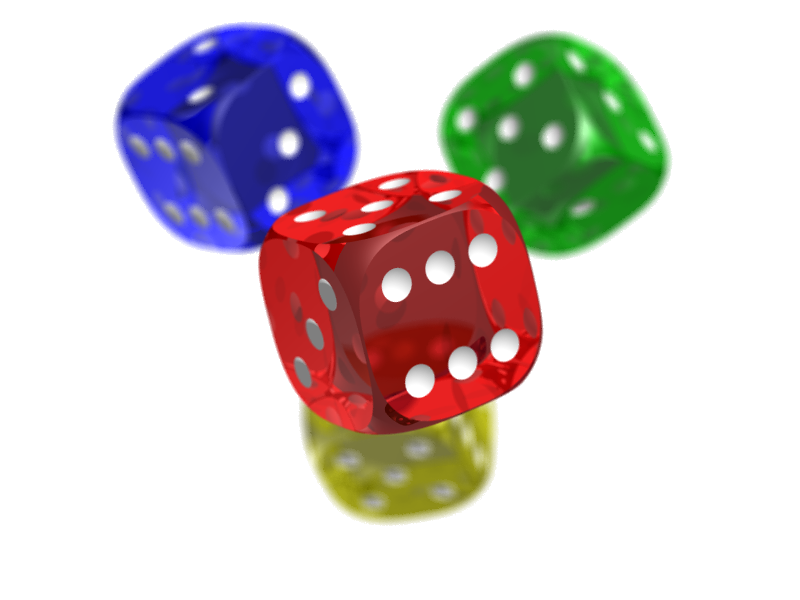
\includegraphics[width=0.4\textwidth]{demo.png}}
					\subfigure[with bg]{\bgbox{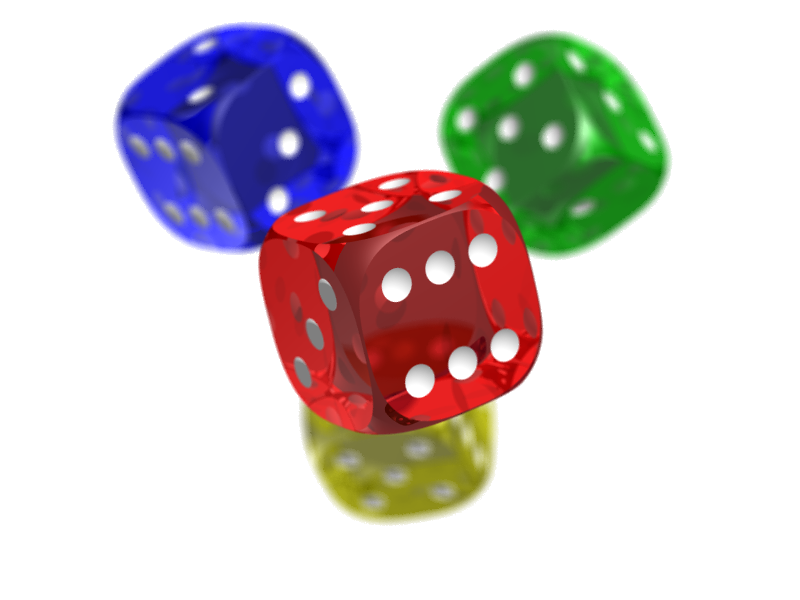
\includegraphics[width=0.4\textwidth]{demo.png}}}
					\caption{This is a graphic taken from \cite{Dice}}
				\end{figure}
		\end{frame}
		
\section{References}
		\begin{frame}
			\frametitle{References}		
				\begin{thebibliography}{99}\small
		\bibitem{Chick}		Chick png from \href{http://commons.wikimedia.org/wiki/File:Chick1.png}{wikimedia: Chick}
		\bibitem{Dice}		Dice PNG from \href{http://commons.wikimedia.org/wiki/File:PNG_transparency_demonstration_1.png}{wikimedia: Dice}
		\bibitem{wikibooks}	Wikibooks on Beamer: \href{http://en.wikibooks.org/wiki/LaTeX/Presentations}{\LaTeX\ presentations}
		\bibitem{userguide}	\href{http://dante.ctan.org/get/macros/latex/contrib/beamer/doc/beameruserguide.pdf}{Beamer user guide}
	 \end{thebibliography}
		\end{frame}



\end{document}
